\originalchapter{15.053 习题课题目与解答}\label{ass:15053-recitations}
本章逐题对应 Spring 2013 的 Recitation 1--10, 助教为 Giacomo Nannicini 与 Ebrahim Nasrabadi. 保留原题号和第一层子问; 同一原编号重复出现时用映射说明区分. “官方解答重构”表示依据官方答案重写并独立核算, “AI 补解/修正”表示补足官方缺答、修正误植或处理原题条件缺口. 数值与换基由附带的 \nolinkurl{tools/audit_lp_recitations.py} 实际运行复核, 计算不以软件输出替代论证. 与第\ref{chap:12}章相同的标准形、换基和灵敏度理论直接沿用该章.

\originalsection{Recitation 1: 建模与凸性}
\begin{exercise}\label{ass:15053-rec1-q1}
原题1. 一家小型配餐企业当天完成烹饪、包装、配送; 配送时间为中午12点至下午2点, 三项工序每天可用时间分别为4、2、2小时. 三种餐点 H（鹰嘴豆泥配饼）、M（慕萨卡）与 T（塔布勒沙拉）的数据如下, 产量允许非整数.
\begin{center}\begin{tabular}{c|rrr}
 &H&M&T\\\hline
烹饪速度（份/小时）&10&5&15\\
包装速度（份/小时）&20&15&25\\
配送速度（份/小时）&30&15&30\\
每份原料成本（美元）&1&2&0.5\\
每份售价（美元）&7&12&5\\
每天订单上限（份）&20&10&30
\end{tabular}\end{center}
\begin{enumerate}[label=(\Alph*)]
\item 写出利润最大的线性规划, 说明变量与约束名称, 并用 Excel 求解（原提示: 最优 M 产量介于5与10）.
\item 弟弟能每天用一小时协助其中一项工序, 效率相同, 可用自行车配送, 工资10美元. 是否聘用? 应分配哪项工序? 分别计算增加一小时的利润变化.
\item H 的订单上限降为10, 最优配餐是否改变? 能否不重新求解就判断?
\item 要求每种餐点都不超过总份数的50\%. 写出新增约束, 判断是否线性, 必要时线性化.
\end{enumerate}
\end{exercise}
\begin{solution}
官方解答重构, 并修正目标方向与零产量说明. (A) 令 $x_H,x_M,x_T$ 为三种份数, 模型为
\begin{align*}
\max\quad&6x_H+10x_M+4.5x_T,\\
\text{烹饪: }&x_H/10+x_M/5+x_T/15\le4,\\
\text{包装: }&x_H/20+x_M/15+x_T/25\le2,\\
\text{配送: }&x_H/30+x_M/15+x_T/30\le2,\\
\text{订单: }&0\le x_H\le20,\quad0\le x_M\le10,\quad0\le x_T\le30.
\end{align*}
最优解 $(8,6,30)$, 利润243美元. 对烹饪、包装、T 订单约束分别乘30、60、0.1并相加, 目标系数恰为 $(6,10,4.5)$, 给上界 $30\cdot4+60\cdot2+0.1\cdot30=243$, 证明最优. 附带脚本用线性规划求解器复算了原要求的电子表格计算.

(B) 增加烹饪、包装、配送各一小时后, 最优方案分别为 $(20,10,25/3)$、$(20,0,30)$、$(8,6,30)$, 利润257.5、255、243, 增量14.5、12、0. 扣工资后净增4.5、2、$-10$, 所以应聘用并协助烹饪. 官方把第三项名称误写为包装, 此处按配送解释.

(C) 原最优 $x_H=8\le10$ 仍可行; 新可行集缩小且包含原最优点, 最优值与该方案都不变.

(D) 用 $2x_i\le x_H+x_M+x_T$（$i=H,M,T$）三条线性约束. 正总产量时它们等价于比例要求; 总产量为0时可约定全部比例限制成立. 线性式本身允许零方案, 官方“相乘后排除零方案”的说法不正确. 原官方模型把利润目标写成 \(\min\), 也与243的正产量答案冲突, 应为 \(\max\).
\end{solution}

\begin{exercise}\label{ass:15053-rec1-q2}
原题2. 四个函数为 $f(x)=x^2/2-5$, $g(x)=x^3/4$, $h(x)=-2\log(x+5)$, $\ell(x)=x^2/2-2\sin x-5$（原图显示区间 $[-4,4]$, $h$ 的自然定义域是 $(-5,\infty)$）.
\begin{enumerate}[label=(\Alph*)]
\item 判断四个函数哪些是凸函数.
\item 判断下列哪些是凸函数: (a) $f+g$; (b) $\pi h$; (c) $2.5f+h$; (d) $\max\{f/3,h/7\}$; (e) $-\ell$.
\end{enumerate}
\end{exercise}
\begin{solution}
官方选择重构, AI 修正其理由. (A) 凸的是 $f,h$: $f''=1$, $h''=2/(x+5)^2>0$; $g''=3x/2$ 在所示区间变号, $\ell''=1+2\sin x$ 也变号. (B) 凸的是 (b)、(c)、(d), 由正倍数、和、逐点最大保持凸性. (a) 的二阶导数 $1+3x/2$ 在 $x<-2/3$ 为负. (e) 的二阶导数 $-1-2\sin x$ 变号, 所以既非凸亦非凹; 官方称其为凹函数不成立. PDF 中该符号是 $\ell$, 文本抽取容易误读为 $f$.
\end{solution}

\begin{exercise}\label{ass:15053-rec1-q3}
原题3. 判断下列规划是否为线性规划; 若不是, 说明能否等价线性化.
\begin{enumerate}[label=(\alph*)]
\item $\min(0.5x_1+3x_2)$, $x_1+1.35x_2=2.7$, $x_1\ge0$, $x_2$ 自由.
\item $\max(0.5x_1+3x_2)$, $0.99x_1+x_2\ge2.7$, $x_1-x_2<8$, $x_1,x_2\ge0$.
\item $\min(0.5x_1+3x_2)$, $(0.99x_1+x_2)/x_2\ge2.7$, $x_1-x_2\le8$, $x_1\ge0$, $x_2$ 自由.
\item 同(c), 但 $x_2\ge1.5$.
\end{enumerate}
\end{exercise}
\begin{solution}
官方分类重构, AI 补充严格等价性. (a) 是 LP, 自由变量不破坏线性. (b) 含严格不等式, 不属于通常以非严格不等式定义的 LP; 不能随意将 $<$ 换成 $\le$ 并声称可行集相同. 本例目标沿 $(t,t)$ 无界, 替换后虽也无界, 但这只说明最优值相同.

(c) 原分式要求 $x_2\ne0$. 若 $x_2<0$, 由 $x_1\ge0$ 得 $0.99x_1/x_2\le0$, 不可能达到1.7. 故可行性实际上强制 $x_2>0$, 分式等价于 $0.99x_1\ge1.7x_2$ 与 $x_2>0$. 该集合不闭: 取 $x_2=\varepsilon$, $x_1=(170/99)\varepsilon$ 趋于原式未定义的原点. 因而不能通过仅含连续变量的普通有限 LP 提升精确表示它. 目标下确界0不取到; 若只写交叉相乘而允许 $x_2=0$, 就错误增加了取到0的解.

(d) 分母严格正, 可等价替为 $0.99x_1\ge1.7x_2$, 其余条件保留, 得 LP.
\end{solution}

\begin{exercise}\label{ass:15053-rec1-q4}
原题4. 有 $m$ 个工厂和 $n$ 个客户, 工厂 $i$ 产能 $p_i$, 客户 $j$ 需求 $d_j$, 单位运输成本 $c_{ij}$. 可运输分数量, 建立满足全部需求、不超过产能的最小成本 LP, 明确变量.
\end{exercise}
\begin{solution}
官方解答重构. 令 $x_{ij}\ge0$ 为工厂 $i$ 运往客户 $j$ 的数量, 则
$\min\sum_{i=1}^m\sum_{j=1}^n c_{ij}x_{ij}$, 条件 $\sum_i x_{ij}=d_j$（每个 $j$）及 $\sum_jx_{ij}\le p_i$（每个 $i$）. 需求等式表示按给定需求配送, 不允许额外配送改变成本.
\end{solution}

\originalsection{Recitation 2: 几何与单纯形}
\begin{exercise}\label{ass:15053-rec2-q1}
原题1. 一个非空二维多面体的顶点依次为 $B,D,F$, 下边界为射线 $BA$、线段 $BD,DF$ 和射线 $FG$, 可行区域向右上无界. $C$ 在 $BD$ 内部, $E$ 在 $DF$ 内部, $A,G$ 分别在两条射线上, $H$ 在可行域内部. 下图独立绘制其关联关系, 不为原图增添数值坐标. 对任意线性目标, 判断下列断言.
\begin{center}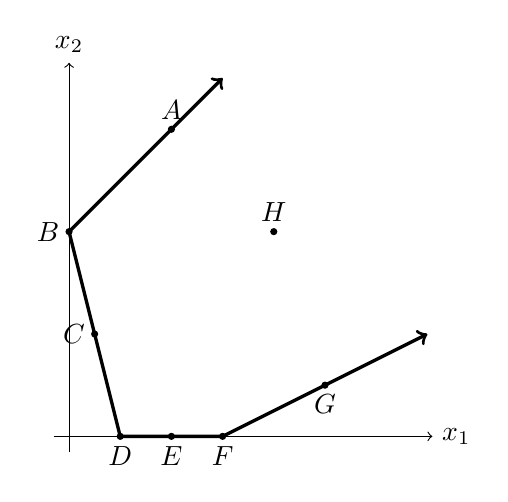
\begin{tikzpicture}[scale=.65]
\draw[->](-.3,0)--(7.1,0) node[right]{$x_1$};\draw[->](0,-.3)--(0,7.3) node[above]{$x_2$};
\draw[very thick,->](0,4)--(3,7);\draw[very thick](0,4)--(1,0)--(3,0);\draw[very thick,->](3,0)--(7,2);
\foreach \x/\y/\l/\p in {0/4/B/left,1/0/D/below,3/0/F/below,.5/2/C/left,2/0/E/below,2/6/A/above,5/1/G/below,4/4/H/above}{\fill (\x,\y) circle(2pt) node[\p]{$\l$};}
\end{tikzpicture}\end{center}
\begin{enumerate}[label=(\alph*)]
\item $F$ 不可能是唯一最优点.
\item 若 $C$ 最优, 则 $D$ 也最优.
\item 若 $A,B$ 最优, 则目标无界.
\item 若 $B,F$ 最优, 则 $G$ 不最优.
\item 若 $B,D,F$ 都不最优, 则目标无界.
\item 存在目标使问题不可行.
\item 若 $B,D,F$ 都不最优, 则问题不可行.
\item $D,F$ 可以同时是仅有的两个最优点.
\item 若 $D,G$ 最优, 则有无穷多个可行点.
\item 即使最优值有限, $G$ 仍可能最优.
\item 存在目标使 $H$ 最优而 $A$ 不最优.
\item 若 $H$ 最优, 则最优解无穷多, 且目标值趋于正或负无穷.
\end{enumerate}
\end{exercise}
\begin{solution}
官方判断重构并补理由. (a) 假, 在 $F$ 两条相邻边法向量之间选择严格支持方向即可唯一最优. (b) 真, 线性目标在 $BD$ 的内部点达到最优时两端同值. (c) 假, 整条射线可以同值最优, 不表示目标值无界. (d) 假, $BF$ 的内部点属于二维可行域内部, 若它最优则目标必须常数, $G$ 也最优. (e) 真, 此无直线的多面体若最优值有限, 必有最优顶点. (f)、(g) 假, 目标不改变已经非空的可行集. (h) 假, 两点最优强制连线段也最优. (i) 真, $DG$ 已含无穷多可行点, 可行域本来也是无界的. (j) 真, 可选择支持射线 $FG$ 的目标. (k) 假, 内点 $H$ 最优迫使目标常数, $A$ 同时最优. (l) 假, 这时目标恒定且有限, 不趋于无穷. 这里“无界”始终指目标无界, 不只是可行区域无界.
\end{solution}

\begin{exercise}\label{ass:15053-rec2-q2}
原题2. 可行集为 $x_1-x_2\ge-1.5$, $x_1-2x_2\le2$, $4x_1+x_2\ge2$, $x_1,x_2\ge0$.
\begin{enumerate}[label=(\alph*)]
\item 画可行域. 每个线性目标都有最优解吗? 为什么?
\item 分别给出: 使 $(0,0),(0,1.5)$ 同时最优的极小目标; 使 $(0,1.5)$ 唯一最优的极小目标; 使目标无界的极大目标. 不存在时解释.
\end{enumerate}
\end{exercise}
\begin{solution}
AI 修正官方漏查可行性. 可行域的三个顶点是 $(1/10,8/5)$、$(1/2,0)$、$(2,0)$; 从第一点沿 $(1,1)$、从第三点沿 $(2,1)$ 向无穷延伸. 可行点位于 $x_2=x_1+3/2$ 的下方, $x_2=(x_1-2)/2$ 与 $x_2=2-4x_1$ 的上方, 并满足非负性.
\begin{center}\begin{tikzpicture}[scale=.7]
\draw[->](0,0)--(5.6,0) node[right]{$x_1$};\draw[->](0,0)--(0,6.6) node[above]{$x_2$};
\draw[very thick,->](.1,1.6)--(4.7,6.2);\draw[very thick](.1,1.6)--(.5,0)--(2,0);\draw[very thick,->](2,0)--(5.2,1.6);
\fill(.1,1.6)circle(2pt) node[left]{$(1/10,8/5)$};\fill(.5,0)circle(2pt) node[below]{$(1/2,0)$};\fill(2,0)circle(2pt) node[below]{$(2,0)$};
\node at(2,2.3){可行域};
\end{tikzpicture}\end{center} $4x_1+x_2\ge2$ 排除了 $(0,0)$ 和 $(0,1.5)$, 后者仅给1.5, 所以(b)前两项都不存在. 官方图与答案未落实这条约束, 不能照搬. 极大目标 $\max x_1$ 沿 $(2,0)+t(2,1)$ 趋于正无穷, 因此(a)答案是否定, (b)末项可用此例.
\end{solution}

\begin{exercise}\label{ass:15053-rec2-q3}
原题3. $\max(10x_1+8x_2-3x_3)$, 约束 $2x_1+4x_2-0.5x_3\le6$, $-2x_1+6x_2-4.5x_3\le4$, $x_1,x_2\ge0$, $x_3$ 自由.
\begin{enumerate}[label=(\alph*)]
\item 转为规范形, 解释新变量, 列出全部变量的初始基本可行解.
\item 列初始单纯形表, 做两次换基, 判断所得解是否最优.
\item 将首约束的 $2x_1$ 改为 $-2x_1$, 列新初表并尝试一次迭代, 说明结果.
\end{enumerate}
\end{exercise}
\begin{solution}
官方解答重构, 修正第二步进入变量名称. (a) 令 $x_3=u-v$, $u,v\ge0$, 加松弛 $s_1,s_2$. 初始 $s_1=6,s_2=4$, 其余变量0. (b) 列顺序 $(x_1,x_2,u,v,s_1,s_2;\mathrm{RHS})$ 的初表为
\[
\begin{pmatrix}10&8&-3&3&0&0&0\\2&4&-1/2&1/2&1&0&6\\-2&6&-9/2&9/2&0&1&4\end{pmatrix}.
\]
首行表示 $-z$ 行. $x_1$ 进入、$s_1$ 离基后为
\[
\begin{pmatrix}0&-12&-1/2&1/2&-5&0&-30\\1&2&-1/4&1/4&1/2&0&3\\0&10&-5&5&1&1&10\end{pmatrix}.
\]
然后是 $v=x_3^-$ 进入, 比值 $3/(1/4)=12$ 与 $10/5=2$, $s_2$ 离基. 终表为
\[
\begin{pmatrix}0&-13&0&0&-51/10&-1/10&-31\\1&3/2&0&0&9/20&-1/20&5/2\\0&2&-1&1&1/5&1/5&2\end{pmatrix}.
\]
所有检验数非正, $(x_1,x_2,x_3)=(5/2,0,-2)$ 最优, 值31. 官方文字把进入列误写 $x_3^+$, 表中实际是 $x_3^-$.

(c) 仅把初表第一约束行的首元素2改为$-2$. 进入 $x_1$ 的两约束列系数均为$-2$, 无离基候选. 射线 $(x_1,x_2,x_3)=(t,0,0)$ 对 $t\ge0$ 可行, 目标 $10t\to\infty$; 算法报告无界, 不会完成普通的有限主元换基.
\end{solution}

\begin{exercise}\label{ass:15053-rec2-q4}
原题4. $\max(2x_1+4x_2)$, $0.5x_1-5x_2\le12$, $x_1+2x_2\ge-2$, $x_2+x_3\ge4$, $x_1,x_2,x_3\ge0$.
\begin{enumerate}[label=(\alph*)]
\item 转规范形, 列初表及初始基本可行解, 注意原变量中至少有一项基本.
\item 选最大正检验数进入, 列离基候选和比值, 写一次换基后的表.
\item 一次迭代后算法会终止吗? 为什么? 最优值如何?
\end{enumerate}
\end{exercise}
\begin{solution}
官方解答重构. 加变量得 $0.5x_1-5x_2+s_1=12$, $-x_1-2x_2+s_2=2$, $x_2+x_3-s_3=4$. 初基 $(s_1,s_2,x_3)=(12,2,4)$, 其余0. 列顺序 $(x_1,x_2,x_3,s_1,s_2,s_3;\mathrm{RHS})$:
\[
T_0=\begin{pmatrix}2&4&0&0&0&0&0\\1/2&-5&0&1&0&0&12\\-1&-2&0&0&1&0&2\\0&1&1&0&0&-1&4\end{pmatrix},
\quad
T_1=\begin{pmatrix}2&0&-4&0&0&4&-16\\1/2&0&5&1&0&-5&32\\-1&0&2&0&1&-2&10\\0&1&1&0&0&-1&4\end{pmatrix}.
\]
$x_2$ 进入, 只有 $x_3$ 的列系数正, 比值4, 故 $x_3$ 离基. 新表中 $s_3$ 检验数4, 约束列系数 $(-5,-2,-1)$ 全非正, 检测无界而终止. 射线 $(x_1,x_2,x_3)=(0,4+t,0)$ 可行, 目标 $16+4t\to\infty$.
\end{solution}

\originalsection{Recitation 3: 多最优解、退化与 Phase I}
\begin{exercise}\label{ass:15053-rec3-q1}
原题1. 极大单纯形初表列为 $(x_1,x_2,x_3,s_1,s_2;\mathrm{RHS})$:
\[
\begin{pmatrix}1&2&5/4&0&0&0\\2&1&1&1&0&6\\0&2&1&0&1&4\end{pmatrix}.
\]
(A) 每次选最大检验数进入, 求最优解与最优值, 判断唯一性. (B) 从终表描述全部最优解, 可先求各最优顶点再给参数方程.
\end{exercise}
\begin{solution}
官方解答重构. (A) 先 $x_2$ 进入、$s_2$ 离开, 后 $x_1$ 进入、$s_1$ 离开, 两表为
\[
\begin{pmatrix}1&0&1/4&0&-1&-4\\2&0&1/2&1&-1/2&4\\0&1&1/2&0&1/2&2\end{pmatrix},\quad
\begin{pmatrix}0&0&0&-1/2&-3/4&-6\\1&0&1/4&1/2&-1/4&2\\0&1&1/2&0&1/2&2\end{pmatrix}.
\]
最优 $(2,2,0)$, 值6. $x_3$ 有零检验数且可增加正步长4, 所以有不同最优点, 并非只凭零检验数判断.

(B) $z=6-s_1/2-3s_2/4$, 最优必须 $s_1=s_2=0$. 令 $x_3=t$, 则全部最优解为 $(x_1,x_2,x_3)=(2-t/4,2-t/2,t)$, $0\le t\le4$, 端点为 $(2,2,0)$ 与 $(1,0,4)$. 从终表让 $x_3$ 进入时 $x_2$ 离开, 得第二端点; 上述等式证明没有别的最优解.
\end{solution}

\begin{exercise}\label{ass:15053-rec3-q2}
原题2. 极大表列为 $(x_1,x_2,x_3,x_4,x_5;\mathrm{RHS})$:
\[
\begin{pmatrix}0&-3&0&2&0&-6\\1&-4&0&2&0&0\\0&-6&1&3&0&2\\0&-1&0&0&1&5\end{pmatrix}.
\]
(A) 给当前基本可行解、目标值与是否退化. (B) 换基一次, 给新解、新值, 与原变量点和表分别比较. (C) 证明无界并给改善目标的可行射线方程.
\end{exercise}
\begin{solution}
官方解答重构. (A) $x=(0,0,2,0,5)$, $z=6$, 基本变量 $x_1=0$, 所以退化. (B) $x_4$ 进入（官方误称 $s_1$）, 比值 $0/2=0,2/3$, $x_1$ 离基, 新表为
\[
\begin{pmatrix}-1&1&0&0&0&-6\\1/2&-2&0&1&0&0\\-3/2&0&1&0&0&2\\0&-1&0&0&1&5\end{pmatrix}.
\]
变量点与值不变, 基与表改变. (C) 令 $x_1=0,x_2=t,x_3=2,x_4=2t,x_5=5+t$, $t\ge0$, 则可行且 $z=6+t\to\infty$.
\end{solution}

\begin{exercise}\label{ass:15053-rec3-q3}
原题3. $\max(x_1+3x_2)$, $2x_1-2x_2=1$, $x_1+x_2\ge5$, $x_1,x_2\ge0$.
(A) 加剩余与人工变量, 给 Phase I 目标、辅助 LP、初表和初始解. (B) 做两次迭代, 判断 Phase I 是否完成, 是否得到原问题的基本可行解并说明.
\end{exercise}
\begin{solution}
官方解答重构. 令剩余 $s_1$, 人工 $s_2,s_3$, 方程 $2x_1-2x_2+s_2=1$, $x_1+x_2-s_1+s_3=5$, 全部非负. 极大辅助目标 $w=-s_2-s_3=3x_1-x_2-s_1-6$. 列顺序 $(x_1,x_2,s_1,s_2,s_3;\mathrm{RHS})$ 的三表为
\[
\begin{pmatrix}3&-1&-1&0&0&6\\2&-2&0&1&0&1\\1&1&-1&0&1&5\end{pmatrix},\quad
\begin{pmatrix}0&2&-1&-3/2&0&9/2\\1&-1&0&1/2&0&1/2\\0&2&-1&-1/2&1&9/2\end{pmatrix},
\]
\[
\begin{pmatrix}0&0&0&-1&-1&0\\1&0&-1/2&1/4&1/2&11/4\\0&1&-1/2&-1/4&1/2&9/4\end{pmatrix}.
\]
初始 $s_2=1,s_3=5$, 其余0. 首步 $x_1$ 进入、$s_2$ 离开; 次步 $x_2$ 进入、$s_3$ 离开. 辅助最优值0, 两人工变量都为0且已离基, 删除其列后 $(x_1,x_2)=(11/4,9/4)$ 为原问题基本可行解, 可恢复原目标进入 Phase II.
\end{solution}

\begin{exercise}\label{ass:15053-rec3-q4}
原题4（原课注明不考的进阶题）. 原变量 $x_1,x_2,x_3\ge0$, 人工变量 $s_1,s_2,s_3$. Phase I 最优值0的表为
\[
\begin{array}{c|rrrrrr|r}
&x_1&x_2&x_3&s_1&s_2&s_3&\mathrm{RHS}\\\hline
-w&0&0&-1&-3&0&-1&0\\
x_1&1&0&2&1&0&2&4\\
x_2&0&1&1&-3&0&5&1\\
s_2&0&0&b&1&1&-1&0
\end{array}
\]
(A) $b=-2$ 时如何使人工变量离基? 给原问题基与可开始 Phase II 的约束表. (B) $b=0$ 时怎么办? 解释末行作为原等式线性组合的意义, 给基与约束表. 原目标未给, 不必写其系数.
\end{exercise}
\begin{solution}
官方解答重构. (A) 用末行 $-2$ 为主元让 $x_3$ 进入、$s_2$ 离开. 虽主元负且该列检验数负, 末行 RHS 为0, 这次代数换基仍保持当前点可行. 人工列删去后约束表是 $I_3x=(4,1,0)\T$, 基为 $(x_1,x_2,x_3)$, 人工变量全部0. 恢复原目标并消去基本列即可.

(B) 末行 $s_1+s_2-s_3=0$, 人工变量去掉后成为 $0=0$, 是冗余原等式. 删此行与全部人工列, 约束表为
$\left(\begin{smallmatrix}1&0&2&4\\0&1&1&1\end{smallmatrix}\right)$, 列为 $(x_1,x_2,x_3;\mathrm{RHS})$, 基 $(x_1,x_2)$, 解 $(4,1,0)$. 原目标未给, 不能把残留的辅助目标行当成 Phase II 的目标行.
\end{solution}

\originalsection{Recitation 4: 灵敏度与活动定价}
\begin{exercise}\label{ass:15053-rec4-q1}
原题1（数学数据的独立重述）. 原习题引用 Bradley、Hax 与 Magnanti 的 \emph{Applied Mathematical Programming}, 第3章题3; 外书背景行文不转载. 以下保留课程给出的模型系数、报告和全部11项数学任务. 记钢、机械、卡车的出口量为 $e_S,e_M,e_T$, 总产量为 $p_S,p_M,p_T$, 都以单位/年计且非负. 模型为
\begin{align*}
\max\quad V={}&900e_S+2500e_M+3000e_T-300p_S-150p_M-500p_T,\\
p_S-.75p_M-p_T-e_S&=0,\\
p_M-.05p_S-.10p_T-e_M&=0,\\
p_T-.08p_S-.12p_M-e_T&=0,\\
p_S\le300000,\quad p_M&\le50000,\quad p_T\le550000,\\
.5p_S+5p_M+3p_T&\le1200000.
\end{align*}
钢的300美元进口成本包括每单位两份100美元矿石与100美元其他材料; 其余进口成本为每机械150、每卡车500美元. 劳动单位为人年. 课程最优报告为出口 $(0,8750,232500)$、总产量 $(300000,50000,262500)$, $V=490625000$美元; 卡车产能余量287500, 劳动余量12500. 平衡等式的影子价格为 $(-2250,-2500,-3000)$; 钢、机械、卡车、劳动产能影子价格为 $(1585,302.5,0,0)$. 钢出口检验数 $-1350$, 售价允许增加1350; 卡车生产成本允许增加1350. 钢、机械产能的允许增加分别为 $25000/7$、$50000/11$, 机械产能允许减少 $350000/43\approx8139.535$. 钢平衡等式 RHS 允许增加232500.
\begin{enumerate}[label=(\alph*)]
\item 从报告解释最佳生产、出口组合, 给单位与净出口价值.
\item 三条平衡等式表示什么? 为什么采用等式?
\item 50000单位机械分别如何使用?
\item 钢售价升至1250美元且选择出口一单位钢时, 净出口价值怎样改变?
\item 新产品使用钢、机械、卡车或劳动四类资源时, 哪类最应节约? 说明使用的资源价格口径.
\item 500000美元投资可增加500单位卡车产能、1000单位机械产能或300单位钢产能, 应选哪个?
\item 每卡车进口材料成本增加400美元时, 最优出口组合与净价值如何?
\item 年末额外库存10000单位钢, 如何改钢平衡式, 净出口价值改变多少?
\item 期初库存 $(S_s,M_s,T_s)$、期末目标库存 $(S_e,M_e,T_e)$, 如何改三条平衡式?
\item 新出口产品每单位使用1.5人年、0.3单位机械, 其售价须达到多少才值得生产?
\item 机械产能降至40000, 依据报告估计净出口价值, 判断是否精确及上/下界方向.
\end{enumerate}
\end{exercise}
\begin{solution}
官方解答重构, (e)、(f)、(k) 加 AI 数学说明. (a) 三种总产量依次300000、50000、262500单位/年, 出口0、8750、232500单位/年, 净出口价值490625000美元. 代入平衡及产能即可验证可行, 给定影子价格满足对偶条件且与该值相等, 故最优.

(b) 产量等于内部使用加出口, 此模型无库存净变化和报废项, 所以物料守恒用等式. (c) 钢生产用 $0.05\cdot300000=15000$ 机械, 卡车生产用 $0.1\cdot262500=26250$, 剩8750出口.

(d) 新钢出口检验数 $-1350+(1250-900)=-1000$. 强制出口一单位而按同一基调整其余产量时, 净价值减少1000至490624000美元; 仅改售价但不强制出口时原方案仍最优.

(e) 必须区别生产能力与中间产品. 若问占用\textbf{产能}, 官方口径选择钢产能, 因其每单位产能影子价格1585高于机械302.5及另两项0. 若新产品直接\textbf{消耗现成钢、机械、卡车}, 正确机会价格来自物料平衡, 分别2250、2500、3000美元, 此口径卡车最高; 不能把钢产能价格1585当成一单位钢的材料价值. 子问(j)使用的2500正是第二口径.

(f) 三种单独增量都在基有效范围内, 毛收益分别 $0\cdot500=0$, $302.5\cdot1000=302500$, $1585\cdot300=475500$. 必须三选一时选钢; 若可以不投资且仅考虑这一年净收益, 三者都不足弥补500000支出.

(g) 最优变量不变, 成本变化在有效范围内; $V=490625000-400\cdot262500=385625000$. (h) 钢平衡 RHS 改10000, 净价值减少 $2250\cdot10000=22500000$, 为468125000. (i) 三条平衡 RHS 分别改 $S_e-S_s,M_e-M_s,T_e-T_s$.

(j) 单位机会成本 $1.5\cdot0+0.3\cdot2500=750$美元; 等于750可达到盈亏平衡, 严格超过750才有严格的边际改善.

(k) 10000的降幅超过允许8139.535, 不能将影子价格变化当精确最优值变化. 原对偶解仍可行, 给上界 $490625000-302.5\cdot10000=487600000$. 官方只扣有效区间内的损失, 得约488162791, 也是更松的上界. AI 重新求解得实际 $V=1399400000/3\approx466466666.67$, 出口 $(0,0,686800/3)$、产量 $(860000/3,40000,770000/3)$. 机械产能与钢/机械零出口平衡确定该点, 劳动仍有余量; 新对偶价格可取平衡 $(-3580/3,-39200/3,-3000)$, 钢/机械/卡车/劳动产能 $(0,34985/3,0,0)$, 其对偶值恰等于上述实际值. 原价格外推是上界, 不保证等号.
\end{solution}

\begin{exercise}\label{ass:15053-rec4-q2}
原题2. $\max(x_1+4x_2)$, 三资源约束 $x_1-x_2\le2$, $x_1+2x_2\le4$, $x_1\le3$, $x_1,x_2\ge0$（非负条件由课程给定的松弛单纯形表体现）. 加松弛 $s_1,s_2,s_3$ 后最优表为
\[
\begin{array}{c|rrrrr|r}&x_1&x_2&s_1&s_2&s_3&\mathrm{RHS}\\\hline
-z&-1&0&0&-2&0&-8\\s_1&3/2&0&1&1/2&0&4\\x_2&1/2&1&0&1/2&0&2\\s_3&1&0&0&0&1&3\end{array}.
\]
(a) 最优解是什么? (b) 各资源影子价格是多少? (c) 分别独立改变 $x_1,x_2$ 的目标系数, 求保持该最优解的范围, 其他数据固定.
\end{exercise}
\begin{solution}
官方解答重构. (a) $(x_1,x_2)=(0,2)$, $(s_1,s_2,s_3)=(4,0,3)$, 值8. (b) 影子价格为 $(0,2,0)$, 由松弛检验数的相反数读取. (c) 非基本 $x_1$ 的系数从1改 $c_1$, 检验数为 $c_1-2$, 所以 $c_1\le2$. 基本 $x_2$ 的系数从4改 $c_2$, 减去其行的 $c_2-4$ 倍使目标行规范化; 非基本 $x_1,s_2$ 检验数分别 $1-c_2/2,-c_2/2$. 故 $c_2\ge2$. 在端点仍保持当前解最优, 可出现其他同值解.
\end{solution}

\begin{exercise}\label{ass:15053-rec4-q3}
原题3. 初表列为 $(x_1,x_2,x_3,x_4,s_1,s_2,s_3;\mathrm{RHS})$:
\[
\begin{pmatrix}3&1&2&-2&0&0&0&0\\1&1&1&1&1&0&0&4\\2&-2&0&-6&0&1&0&2\\3&0&1&-1&0&0&1&7\end{pmatrix},
\]
末行基本变量原表误标 $s_2$, 按单位列应为 $s_3$. 给定最优表为
\[
\begin{pmatrix}0&0&0&-1&-2&-1/2&0&-9\\0&0&1&-4&3&3/2&-2&1\\1&0&0&1&-1&-1/2&1&2\\0&1&0&4&-1&-1&1&1\end{pmatrix}.
\]
(a) 给最优解. (b) 求各约束影子价格. (c) 新活动使用资源列 $(0.5,2,5)\T$, 求盈亏平衡单位收入. (d) $x_4$ 的目标系数最多可增加多少而保持原解最优?
\end{exercise}
\begin{solution}
官方重构并 AI 修正(b). (a) $(x_1,x_2,x_3,x_4)=(2,1,1,0)$, 松弛全0, 值9. (b) 正确价格 $(2,1/2,0)$, 官方的 $(0.5,0,9)$ 是误复制. (c) 价格内积 $2\cdot0.5+0.5\cdot2+0\cdot5=2$, 收入2为盈亏平衡, 超过2才严格改善. (d) $x_4$ 非基本且检验数$-1$, 最多增加1, 即由$-2$增至$-1$; 等号时当前解仍最优.
\end{solution}

\originalsection{Recitation 5: Phase I 与零和博弈}
\begin{exercise}\label{ass:15053-rec5-q1}
原题1. 初始表为
\[
\begin{array}{c|rrrrrrr|r}&x_1&x_2&x_3&x_4&s_1&s_2&s_3&\mathrm{RHS}\\\hline
-z&2&3&5&2&0&0&0&0\\s_1&5&6&-1&2&1&0&0&6\\s_2&-3&-1&2&-1&0&1&0&4\\s_3&-2&0&2&-2&0&0&1&3
\end{array}.
\]
三次换基后约束行基本变量为 $x_4,x_3,s_3$, 右端 $(16/3,14/3,13/3)$, 目标行松弛系数 $(-3,-4,0)$, $x_1,x_2,x_3,x_4$ 系数缺失为 $a,b,c,d$, RHS 缺失为 $e$. 约束行的全部系数为
\[\begin{pmatrix}1&11/3&0&1&2/3&1/3&0&16/3\\-1&4/3&1&0&1/3&2/3&0&14/3\\2&14/3&0&0&2/3&-2/3&1&13/3\end{pmatrix}.\]
(a) 求单纯形乘子与 $a,b,c,d,e$. (b) $x_2$ 目标系数从3增至8, 原解仍最优吗?
\end{exercise}
\begin{solution}
官方解答重构. 乘子 $\pi=(3,4,0)$, 约化成本 $c_j-\pi a_j$ 给 $(a,b,c,d)=(-1,-11,0,0)$; 最优值 $2(16/3)+5(14/3)=34$, 所以 $e=-34$. $x_2$ 非基本, 其系数增加5后检验数$-6\le0$, 其他不变, 原解仍最优. 允许增加包含端点11, 官方“少于11”可放宽为“不超过11”.
\end{solution}

\begin{exercise}\label{ass:15053-rec5-q2}
原题2. $\max(x_1-2x_2)$, $3x_1+x_2\ge3$, $x_1+2x_2=4$, $x_1,x_2\ge0$.
(a) 转标准形. (b) 写构造初始可行基的 Phase I 问题. (c) 列规范初表, 新增变量最多3个, 目标行 RHS 必须正确.
\end{exercise}
\begin{solution}
官方解答重构. (a) 第一约束减剩余 $s_1\ge0$: $3x_1+x_2-s_1=3$. (b) 两行加人工 $w_1,w_2\ge0$, 方程 $3x_1+x_2-s_1+w_1=3$, $x_1+2x_2+w_2=4$, 辅助目标 $\max(-w_1-w_2)=\max(4x_1+3x_2-s_1-7)$. (c) 列 $(x_1,x_2,s_1,w_1,w_2;\mathrm{RHS})$ 的规范初表为
$\left(\begin{smallmatrix}4&3&-1&0&0&7\\3&1&-1&1&0&3\\1&2&0&0&1&4\end{smallmatrix}\right)$, 初基 $w_1=3,w_2=4$, 其余0. 目标行 RHS 为7, 因初始辅助目标为$-7$.
\end{solution}

\begin{exercise}\label{ass:15053-rec5-q3}
原题3. 两人零和博弈, 行玩家收益矩阵为
$A=\left(\begin{smallmatrix}2&3&-2\\3&1&0\\-3&-3&3\end{smallmatrix}\right)$.
(a) 建立行玩家最优混合策略 LP, 不必求解. (b) 建立列玩家最优混合策略 LP, 不必求解.
\end{exercise}
\begin{solution}
官方结构重构, AI 修正矩阵系数. (a) 令行概率 $x_i\ge0$, $\sum_ix_i=1$, 收益下界 $v$ 自由, 最大化 $v$, 约束
$v\le2x_1+3x_2-3x_3$, $v\le3x_1+x_2-3x_3$, $v\le-2x_1+3x_3$.
(b) 令列概率 $y_j\ge0$, $\sum_jy_j=1$, 上界 $w$ 自由, 最小化 $w$, 约束 $w\ge2y_1+3y_2-2y_3$, $w\ge3y_1+y_2$, $w\ge-3y_1-3y_2+3y_3$. 约束各自防范对方所有纯策略, 混合策略为纯策略期望的凸组合, 因此足够. 官方中间写概率 $\ge1$, 以及行模型末项 $x_3$ 缺系数3, 都不符合题给矩阵.
\end{solution}

\begin{exercise}\label{ass:15053-rec5-q4}
原题4. 两人同时喊1或2. 行玩家 Odd 在数字之和为奇数时赢, 列玩家 Even 在和为偶数时赢, 败者支付数字之和（美元）. 谁占优势?
\end{exercise}
\begin{solution}
官方结果重构并修正极值方向. Odd 收益矩阵为 $\left(\begin{smallmatrix}-2&3\\3&-4\end{smallmatrix}\right)$. 若 Odd 以概率 $p$ 喊1, 两种列选择收益为 $3-5p,7p-4$, 应求 $\max_{0\le p\le1}\min\{3-5p,7p-4\}$. 相交于 $p=7/12$, 值 $1/12$; 左侧较小收益递增, 右侧较小收益递减, 故为最优. Even 也以概率 $7/12$ 喊1使行玩家两行期望相等, 证明双方最优及 Odd 每次平均占 $1/12$ 美元优势. 官方的 $\min\max$ 是极值方向误植.
\end{solution}

\originalsection{Recitation 6: 整数模型与分段线性函数}
\begin{exercise}\label{ass:15053-rec6-q1}
原题1. 整数规划 $\max c\T x$, $c=(21,32,40,49,57,71,82,91,100,109)\T$, 资源约束 $\sum_{i=1}^{10}(i+1)x_i\le900$, $x_1,x_2,x_3\in\{0,1\}$, 其余 $x_i$ 为 $[0,100]$ 中整数. 原显示式未重复后七项的整数声明, 以下按题名与分段整数区间的原意解释. 每小问独立, 只写新增变量和约束.
\begin{enumerate}[label=(\alph*)]
\item 用一条线性约束表示“$x_1=1$ 则 $x_2=0$”.
\item 用一条约束表示“$x_2=1$ 或 $x_3=0$, 但不能两者都成立”.
\item 加二元 $w_1$ 与两条约束, 使 $x_5+x_6\ge70$ 时 $w_1=1$, $x_5+x_6\le69$ 时 $w_1=0$.
\item 加三二元 $w_2,w_3,w_4$ 与至多四约束, 确保 $x_5\le92$, $x_6\le40$, $x_7+x_8\ge74$ 中至少一条成立.
\item 加一二元 $w_5$ 与两约束, 确保 $x_9\le45$ 或 $x_{10}\ge22$.
\item 加一整数 $w_6$ 与一约束, 使 $x_8$ 除4余2.
\item 加三二元 $w_7,w_8,w_9$ 与两约束, 使 $x_{10}\in\{13,39,88\}$.
\item 表示成本 $f_4(0)=0$, $f_4(x_4)=250+49x_4$（$x_4\ge1$）.
\item 表示成本 $f_5(x_5)=57x_5$（$0\le x_5\le10$）, $570$（$11\le x_5\le20$）, $-480+50x_5$（$21\le x_5\le100$）.
\end{enumerate}
原分数为(a)--(h)各4分、(i)8分.
\end{exercise}
\begin{solution}
官方结构重构并给有效有限常数. (a) $x_1+x_2\le1$. (b) $x_2=x_3$, 恰允许 $(x_2,x_3)=(0,0),(1,1)$. (c) $70w_1\le x_5+x_6\le69+131w_1$. 整数性保证70与69之间无遗漏整数; 若后七项允许连续, 原两个条件对 $(69,70)$ 的值不作要求, 不能称同一双向阈值逻辑.

(d) $x_5\le92+8(1-w_2)$, $x_6\le40+60(1-w_3)$, $x_7+x_8\ge74-74(1-w_4)$, $w_2+w_3+w_4\ge1$. (e) $x_9\le45+55w_5$, $x_{10}\ge22-22(1-w_5)$. (f) $x_8=4w_6+2$, $w_6$ 整数; 原界自动给 $0\le w_6\le24$. (g) $x_{10}=13w_7+39w_8+88w_9$, $w_7+w_8+w_9=1$.

(h) 加二元 $u$, $u\le x_4\le100u$, 成本变量 $t_4=250u+49x_4$. 若原目标将49$x_4$作为收益, 把新成本项纳入目标时须按所建经济模型说明符号, 不能默认重复计入同一49$x_4$.

(i) 加二元 $u_1,u_2,u_3$, 非负 $y_1,y_2,y_3$, $\sum_ku_k=1$, $x_5=\sum_ky_k$, $0\le y_1\le10u_1$, $11u_2\le y_2\le20u_2$, $21u_3\le y_3\le100u_3$, 成本 $t_5=57y_1+570u_2-480u_3+50y_3$. 恰选一段, 未选段的 $y_k=0$, 已选段 $y_k=x_5$, 故成本等式在每个允许整数值都正确.
\end{solution}

\begin{exercise}\label{ass:15053-rec6-q2}
原题2. 从10处勘探点 $S_1,\ldots,S_{10}$ 中恰选5处, 每处成本 $c_j$, 最小化总成本, 仅用二元变量 $x_j$ 表示选择. 要求: (i) 同选 $S_2,S_7$ 时不能选 $S_6,S_9$ 的任何一个; (ii) 同选 $S_1,S_3$ 时不能又同时选 $S_5,S_6$; (iii) 选 $S_3$ 或 $S_4$ 时不得选 $S_6$; (iv) $S_3,S_6,S_7,S_8$ 至多选两个. 建整数规划.
\end{exercise}
\begin{solution}
官方结构重构, AI 修正选择数与严格号误植. 目标 $\min\sum_jc_jx_j$, $\sum_jx_j=5$, $x_j\in\{0,1\}$. 新增
\[
\begin{aligned}
&x_2+x_7+x_6\le2,\quad x_2+x_7+x_9\le2,\\
&x_1+x_3+x_5+x_6\le3,\\
&x_3+x_6\le1,\quad x_4+x_6\le1,\\
&x_3+x_6+x_7+x_8\le2.
\end{aligned}
\]
每式恰排除相应禁止组合. 官方误写 $\sum c_jx_j=5$ 以及最后 $<2$, 均不符合题意. 脚本已对 $2^{10}=1024$ 个二元组合逐一比对逻辑条件与上述线性条件.
\end{solution}

\begin{exercise}\label{ass:15053-rec6-q3}
原题3. 图中分段线性函数由直线 $4-x$, $1+x/2$, $-5+2x$ 的上包络组成, 折点 $(2,2),(4,3)$, 图示部分为 $(0,4)$ 至 $(6,7)$. 变量 $x$ 与其他变量还满足一组线性约束, 因此不能仅看图决定其值.
\begin{center}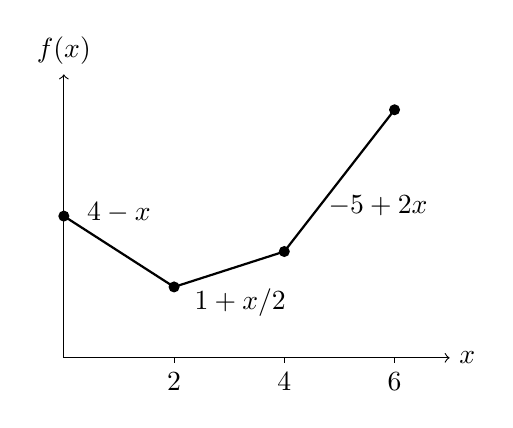
\begin{tikzpicture}[x=.7cm,y=.45cm]
\draw[->](0,0)--(7,0) node[right]{$x$};\draw[->](0,0)--(0,8) node[above]{$f(x)$};
\draw[thick](0,4)--(2,2)--(4,3)--(6,7);
\foreach \x/\y in {0/4,2/2,4/3,6/7}{\fill(\x,\y) circle(2pt);}
\node at(1,4.1){$4-x$};\node at(3.2,1.55){$1+x/2$};\node at(5.7,4.3){$-5+2x$};
\foreach \x in {2,4,6}{\draw(\x,0)--(\x,-.15) node[below]{$\x$};}
\end{tikzpicture}\end{center}
(a) 将最小化 $f(x)$ 写成线性模型, 是否需要整数变量? 可不写其他线性约束. (b) 为什么不能同样处理最大化? 给一个替代模型, 必要时加二元或整数变量.
\end{exercise}
\begin{solution}
官方上图模型重构, AI 修正最大化说明与界条件. (a) 令 $t\ge4-x$, $t\ge1+x/2$, $t\ge-5+2x$, 最小化 $t$, 不需整数变量. 在最优处 $t=f(x)$, 其余原约束保留. 不需要额外强制 $t\ge0$ 或 $x\ge0$, 除非原定义域确已给出.

(b) 最大化同一个上图变量 $t$ 会允许其无界增大. 但有一个不添加任何界的可靠方法: 对同一原可行集分别最大化三条仿射式, 再取三个最优值的最大值, 因为 $\sup_x\max_k\ell_k(x)=\max_k\sup_x\ell_k(x)$. 每个子问题都是 LP, 不需整数变量.

若要求一份选择分段的整数模型, 且按原图所示范围明确采用 $0\le x\le6$, 可令二元 $u_1,u_2,u_3$ 恰一项为1, $x=y_1+y_2+y_3$, $0\le y_1\le2u_1$, $2u_2\le y_2\le4u_2$, $4u_3\le y_3\le6u_3$, 最大化 $4u_1-y_1+u_2+y_2/2-5u_3+2y_3$. 边界处相邻表达式同值, 故选哪段都正确. 若原附加约束还允许图外 $x$, 不能悄悄把6作为上界; 应采用前述三个 LP 或从真实界重新构造分段模型. 官方说明曾把区间写为 $[0,3)$、将 $u_2=1$ 误写成2、并把凸/凹函数的优化方向颠倒, 均以本解的等价性检验为准.
\end{solution}

\originalsection{Recitation 7: 分支定界}
\begin{exercise}\label{ass:15053-rec7-q1}
原题1. 极大0--1规划节点11中前三变量已固定, 可行整数当前最好值15, 下一步对 $x_4$ 分支至节点12（$x_4=1$）和13（$x_4=0$）. 节点11图示 LP 值16, 模型为
$\max(18x_4+ax_5+10)$, $8x_4+10x_5\le5$, $0\le x_4,x_5\le1$.
(A) $x_4=1$ 时节点12应剪枝吗? (B) $x_4=0,a=12$ 时节点13应剪枝吗? (C) $x_4=0,a=8$ 时呢? 解释.
\end{exercise}
\begin{solution}
官方解答重构. (A) $10x_5\le-3$ 与 $x_5\ge0$ 冲突, 不可行剪枝. (B) $x_5\le1/2$, LP 解 $x_5=1/2$, 上界16高于15且非整数, 普通分支定界暂不剪枝. (C) LP 上界14不超过15, 按界剪枝. 原图节点11的16与给出的完整模型不一致: 对 $a=12$ 或8, 根 LP 至少允许 $(x_4,x_5)=(5/8,0)$, 值21.25. 子节点判断仅依赖明确模型与当前最好值, 不采用该错误的父节点标签. 因剩余只含一个二元变量, 还可用额外整数推理提前判断 $x_5=0$, 但(B)按原题所问的 LP 剪枝规则回答.
\end{solution}

\begin{exercise}\label{ass:15053-rec7-q2}
原题2. 原题显示目标 $\max(x_4+5x_2)$, 约束 $-4x_1+3x_2\le6$, $3x_1+2x_2\le18$, $x_1,x_2\ge0$ 且整数. $x_4$ 在其他条件中未定义.
(A) 在平面画出整数可行解集. (B) 用几何法解每个 LP 松弛, 完成分支定界并解释几何过程. 以下另列 AI 明确修正版: 将目标中的 $x_4$ 改为 $x_1$, 其他条件不变; 原官方答案漏了整题.
\end{exercise}
\begin{solution}
AI 补解, 不声称修正版是原题唯一意图. 若将 $x_4$ 当独立无上界变量, 原目标无界; 若不定义它, 原问题不完整. 修正版的整数点可精确列为
\[
\begin{aligned}
&\{(0,j):0\le j\le2\}\cup\{(1,j):0\le j\le3\}\cup\{(2,j):0\le j\le4\}\\
&{}\cup\{(3,j):0\le j\le4\}\cup\{(4,j):0\le j\le3\}\\
&{}\cup\{(5,j):0\le j\le1\}\cup\{(6,0)\}
\end{aligned}.
\]
\begin{center}\begin{tikzpicture}[scale=.58]
\draw[->](0,0)--(6.8,0) node[right]{$x_1$};\draw[->](0,0)--(0,6.4) node[above]{$x_2$};
\draw[dashed](0,0)--(6,0)--(2.4705882353,5.2941176471)--(0,2)--cycle;
\foreach \x in {2,3,4}{\draw[gray,densely dashed](\x,0)--(\x,6);}
\foreach \y in {4,5}{\draw[gray,dotted](0,\y)--(6,\y) node[right]{$x_2=\y$};}
\fill[structurecolor](2,4.6666666667)circle(2.3pt) node[above left]{$L$};
\fill[structurecolor](3,4.5)circle(2.3pt) node[above right]{$R$};
\fill[structurecolor](3.3333333333,4)circle(2.3pt) node[below right]{$R_0$};
\foreach \x/\u in {0/2,1/3,2/4,3/4,4/3,5/1,6/0}{\foreach \y in {0,...,\u}{\fill(\x,\y)circle(2pt);}}
\draw[structurecolor,very thick](3,4)circle(4pt);\node[above right]at(3,4){整数最优 $(3,4)$};
\fill(2.4705882353,5.2941176471)circle(2pt);\node[above]at(2.4705882353,5.2941176471){LP 最优};
\foreach \x in {1,...,6}{\node[below]at(\x,0){$\x$};}\foreach \y in {1,...,5}{\node[left]at(0,\y){$\y$};}
\end{tikzpicture}\end{center}
根 LP 顶点 $(0,0),(6,0),(42/17,90/17),(0,2)$; 最优交点 $(42/17,90/17)$, 值 $492/17$. 对 $x_1\le2$、$x_1\ge3$ 分支, 分别求得 $(2,14/3)$、$(3,9/2)$, 上界 $76/3,51/2$.

左节点再分 $x_2\le4$、$x_2\ge5$, 前者最优 $(2,4)$ 值22为整数, 后者不可行. 右节点同样分, $x_2\ge5$ 不可行, $x_2\le4$ 的 LP 解 $(10/3,4)$ 值 $70/3$. 图中灰虚线为竖直分支线 $x_1=2,3,4$ 与水平分支线 $x_2=4,5$, $L,R,R_0$ 分别标左子、右子及右子加 $x_2\le4$ 后的 LP 最优点. 将后者分为 $x_1\le3$ 与 $x_1\ge4$, 得整数解 $(3,4)$ 值23、$(4,3)$ 值19, 剪枝后无活跃节点, 故整数最优23. 几何上每次分支删去两相邻整数水平/竖直线之间的开条带, 松弛边界交点给各节点上界.
\end{solution}

\begin{exercise}\label{ass:15053-rec7-q3}
原题3. 背包 $\max(19x_1+23x_2+30x_3+40x_4)$, $6x_1+8x_2+10x_3+13x_4\le25$, $x_i\in\{0,1\}$. 用分支定界求解; 一约束 LP 松弛可按单位重量收益填装.
\end{exercise}
\begin{solution}
AI 修正官方节点值与整数总收益. 单位重量收益降序为 $19/6>40/13>30/10>23/8$. 根松弛 $(1,0,3/5,1)$ 值77, 分数变量 $x_3$ 分支. 以下按深度优先列完整树的叶子与待分节点, 固定条件均累积于父条件; 最初当前最好值0.
\begin{center}\begin{tabular}{l|r|l}
固定条件&LP 上界&处理\\\hline
无&77&分 $x_3$\\
$x_3=0$&$305/4$&分 $x_2$\\
$x_3=0,x_2=0$&59&整数 $(1,0,0,1)$\\
$x_3=0,x_2=1$&$986/13$&分 $x_4$\\
上述 $x_4=0$&42&界剪枝\\
上述 $x_4=1$&$227/3$&分 $x_1$\\
上述 $x_1=0$&63&整数 $(0,1,0,1)$\\
上述 $x_1=1$&不可行&剪枝\\
$x_3=1$&$997/13$&分 $x_4$\\
$x_3=1,x_4=0$&72&整数 $(1,1,1,0)$\\
$x_3=1,x_4=1$&$229/3$&分 $x_1$\\
上述 $x_1=1$&不可行&剪枝\\
上述 $x_1=0$&$303/4$&分 $x_2$\\
上述 $x_2=0$&70&界剪枝\\
上述 $x_2=1$&不可行&剪枝
\end{tabular}\end{center}
所有叶子都已封闭, 最好整数方案 $(1,1,1,0)$ 重量24、收益72. 官方将 $19+23+30$ 写成73, 根 LP 写成75.75, 都与题给系数不符. 此题在官方解答中误标 Problem 2, 本章按原题面映射为 Problem 3.
\end{solution}

\originalsection{Recitation 8: 整数凸包与割平面}
\begin{exercise}\label{ass:15053-rec8-q1}
原题1. 原图整数可行点经逐点核实为 $(2,1),(3,1),(3,2),(4,1),(4,2),(4,3),(5,2)$. 下图独立绘出这些数学数据; 原图中的连续多边形只用于对比, 有效不等式以全部整数点为准. 判断 (a) $x\le4$; (b) $x\ge2$; (c) $y\ge1$; (d) $y\le6$; (e) $x+y\ge3$ 哪些有效.
\begin{center}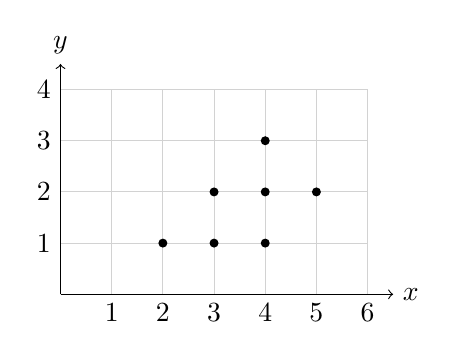
\begin{tikzpicture}[scale=.65]
\draw[step=1,gray!35] (0,0) grid (6,4);\draw[->](0,0)--(6.5,0) node[right]{$x$};\draw[->](0,0)--(0,4.5) node[above]{$y$};
\foreach \x/\y in {2/1,3/1,3/2,4/1,4/2,4/3,5/2}{\fill(\x,\y)circle(2.5pt);}
\foreach \x in {1,...,6}{\node[below]at(\x,0){$\x$};}\foreach \y in {1,...,4}{\node[left]at(0,\y){$\y$};}
\end{tikzpicture}\end{center}
\end{exercise}
\begin{solution}
官方判断重构. (a) 无效, 点 $(5,2)$ 违反; (b)--(e) 全有效, 点集中 $x\ge2,y\ge1$, 最大 $y=3\le6$, 最小 $x+y=3$. 原题(d)行自带 ``Yes'', 本章仍保留其数学判断任务.
\end{solution}

\begin{exercise}\label{ass:15053-rec8-q2}
原题2. 整数集 $F$ 由 $-3x_1+5x_2\le12$, $4x_1+3x_2\le20$, $x_1+x_2\le11/2$, $x_1,x_2\ge0$ 且整数定义.
(a) 画 LP 松弛, 求整数点凸包, 先从图识别再给定义不等式. 原提示两斜线分别过 $(-4,0),(1,3)$ 和 $(5,0),(2,4)$.
(b) 对 $X=\{(x_1,x_2)\in\mathbb Z^2:x_1+x_2\le11/2\}$, 判断 $F,X$ 的包含关系, 给 $X$ 的有效不等式并说明为何对 $F$ 也有效.
\end{exercise}
\begin{solution}
官方解答重构并精确核点. LP 顶点为 $(0,0),(5,0),(7/2,2),(31/16,57/16),(0,12/5)$. 图中虚线为松弛边界, 实线为整数凸包.
\begin{center}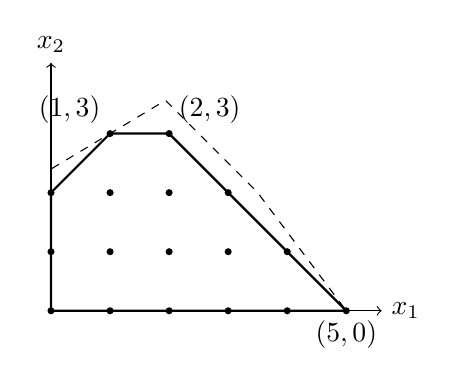
\begin{tikzpicture}[scale=.75]
\draw[->](0,0)--(5.6,0) node[right]{$x_1$};\draw[->](0,0)--(0,4.2) node[above]{$x_2$};
\draw[dashed](0,0)--(5,0)--(3.5,2)--(1.9375,3.5625)--(0,2.4)--cycle;
\draw[thick](0,0)--(5,0)--(2,3)--(1,3)--(0,2)--cycle;
\foreach \x/\y in {0/0,0/1,0/2,1/0,1/1,1/2,1/3,2/0,2/1,2/2,2/3,3/0,3/1,3/2,4/0,4/1,5/0}{\fill(\x,\y)circle(1.7pt);}
\node[above right]at(2,3){$(2,3)$};\node[above left]at(1,3){$(1,3)$};\node[below]at(5,0){$(5,0)$};
\end{tikzpicture}\end{center}
凸包为 $x_1,x_2\ge0$, $-x_1+x_2\le2$, $x_2\le3$, $x_1+x_2\le5$. 枚举17个整数点后, 极点恰为 $(0,0),(5,0),(2,3),(1,3),(0,2)$; 它们都属于 $F$, 给出的多边形包含所有整数点, 所以恰等于 $\conv F$. (b) $F\subsetneq X$, 例如 $(-1,0)\in X\setminus F$. 整数和 $x_1+x_2\le5.5$ 等价于 $\le5$, 因此 $x_1+x_2\le5$ 对 $X$ 有效, 对其子集 $F$ 也有效.
\end{solution}

\begin{exercise}\label{ass:15053-rec8-q3}
原题3. 所有变量包括松弛均非负整数, 极大 LP 松弛初表列为 $(x_1,x_2,x_3,s_1,s_2,s_3;\mathrm{RHS})$:
\[
\begin{pmatrix}-2&4&1&0&0&0&0\\2&1&1&1&0&0&8\\-4&4&2&0&1&0&8\\1&2&3&0&0&1&9\end{pmatrix}.
\]
给定最优基为 $(s_1,x_2,x_1)$, 最优表为
\[
\begin{pmatrix}0&0&-7/3&0&-2/3&-2/3&-34/3\\0&0&-3/2&1&1/4&-1&1\\0&1&7/6&0&1/12&1/3&11/3\\1&0&2/3&0&-1/6&1/3&5/3\end{pmatrix}.
\]
(a) 从最后两条约束各推导一条 Gomory 割. (b) 当前基本解满足任一割吗?
\end{exercise}
\begin{solution}
AI 修正官方首割的系数. 由 $x_2+(7/6)x_3+(1/12)s_2+(1/3)s_3=11/3$, 将系数和 RHS 向下取整给 $x_2+x_3\le3$（非负整数变量使左端整数且不超过11/3）; 用原等式减去该不等式, 得
\[
\tfrac16x_3+\tfrac1{12}s_2+\tfrac13s_3\ge\tfrac23.
\]
另一行 $x_1+(2/3)x_3-(1/6)s_2+(1/3)s_3=5/3$, 取整得 $x_1-s_2\le1$, 相减得
\[
\tfrac23x_3+\tfrac56s_2+\tfrac13s_3\ge\tfrac23.
\]
当前解 $(x_1,x_2,x_3,s_1,s_2,s_3)=(5/3,11/3,0,1,0,0)$ 对两割左边都为0, 均违反. 官方首割把 $x_3$ 分数部分写成1/3, 应为 $7/6-1=1/6$, 此处从初矩阵与基独立重算了全部终表.
\end{solution}

\begin{exercise}\label{ass:15053-rec8-q4}
原题4. $K=\{x\in\{0,1\}^7:11x_1+6x_2+6x_3+5x_4+5x_5+4x_6+x_7\le19\}$.
(a) 判断以下是否有效覆盖不等式并解释: (a) $x_4+x_5+x_6\le2$; (b) $x_1+x_2+x_6\le2$; (c) $x_2+x_3+x_6+x_7\le3$; (d) $x_2+x_4+x_5+x_6\le3$; (e) $x_1+x_3+x_4+x_5\le3$; (f) $x_2+x_3+x_4+x_5+x_6\le4$.
(b) 有效覆盖中哪些最小?
(c) 进阶: 将 $x_2+x_3+x_4+x_5\le3$ 在 RHS 不变下加入更多变量, 求一条扩展覆盖并比较强弱.
\end{exercise}
\begin{solution}
官方解答重构, AI 加严格强弱证据. 覆盖 $C$ 有效当且仅当总重量超过19; 最小覆盖要求删任何项后都不超过19. 六集合重量依次14、21、17、20、27、26, 所以有效者为(b)、(d)、(e)、(f), 其中(b)、(d)最小, (e)、(f)非最小: (e)删一项重量5后仍22, (f)删项6的重量4后仍22.

(c) $x_1+x_2+x_3+x_4+x_5\le3$ 有效, 因这五项中最轻的四项重量 $5+5+6+6=22>19$. 由 $x_1\ge0$, 它蕴含原覆盖, 且在 LP 松弛上严格更强: 取 $(x_1,x_2,x_3,x_4,x_5,x_6,x_7)=(1/8,3/4,3/4,3/4,3/4,0,0)$, 重量 $143/8=17.875\le19$, 原覆盖和3满足, 新覆盖和 $25/8>3$ 违反. 官方所举全五项 $3/4$ 的点本身超过背包容量, 本解提供了仍在原 LP 松弛内的反例.
\end{solution}

\originalsection{Recitation 9: 最短路与网络流}
本节原题顺序为1、3、3、5, 以下依次映射为1、3(a)、3(b)、5; 括号用于区分重复原号, 不改变题内子问编号.
\begin{exercise}\label{ass:15053-rec9-q1}
原题1. 有向弧及长度为 $SA:1$, $SB:6$, $SC:3$, $AD:6$, $AB:4$, $BD:1$, $BT:5$, $CE:2$, $DT:2$, $ET:4$. 一次 Dijkstra 迭代包含选一个永久节点并扫描其出弧. 已做两次, 永久集合 $\{S,A\}$, 距离按 $(S,A,B,C,D,E,T)$ 为 $(0,1,5,3,7,\infty,\infty)$. 再做一次, 给全部永久状态与距离.
\begin{center}\begin{tikzpicture}[>=Stealth,x=1.4cm,y=.8cm]
\foreach \n/\x/\y in {S/0/0,A/1/1.5,C/1/-1.5,B/2/0,D/3/1.5,E/3/-1.5,T/4/0}{\node[draw,circle,inner sep=3pt](\n)at(\x,\y){$\n$};}
\foreach \a/\b/\w in {S/A/1,S/B/6,S/C/3,A/D/6,A/B/4,B/D/1,B/T/5,C/E/2,D/T/2,E/T/4}{\draw[->](\a)--(\b) node[midway,fill=white,inner sep=1pt]{$\w$};}
\end{tikzpicture}\end{center}
\end{exercise}
\begin{solution}
官方解答重构. 未永久节点中 $C$ 距离3最小, 将 $C$ 永久化, 扫描 $CE$ 得 $d_E=\min(\infty,3+2)=5$. 新永久集合 $\{S,A,C\}$, 距离 $(0,1,5,3,7,5,\infty)$. 不在同一迭代继续扫描尚未永久的 $E$.
\end{solution}

\begin{exercise}\label{ass:15053-rec9-q3a}
原题3(a), 即第一个 Problem 3. Boston、Raleigh 年产能分别400、300台电脑, 单位生产成本800、900美元. Los Angeles 需求400, Austin 需求300, 可经 Chicago 转运. 单位运费（美元）:
\begin{center}\begin{tabular}{c|rrr}出发地&Chicago&Austin&Los Angeles\\\hline
Boston&80&220&280\\Raleigh&100&140&170\\Chicago&---&40&50
\end{tabular}\end{center}
(a) 建立包含生产与运输成本的最小费用流模型. (b) 至多200台经 Chicago 时怎样修改? (c) Raleigh 产能为500时怎样修改网络, 并说明处理供给多余的一般方法.
\end{exercise}
\begin{solution}
官方网络结构重构并补足(c)的容量口径. (a) 增虚拟源 $s$, 弧 $s\to B$ 费用800容量400, $s\to R$ 费用900容量300; 其余弧按运费表且无额外容量上限. 正供给定义为流出减流入, 节点 $s$ 供给700, $L,A$ 供给分别$-400,-300$, 其余0. 变量 $f_{ij}\ge0$, 最小化 $\sum c_{ij}f_{ij}$, 每节点满足 $\sum_jf_{ij}-\sum_jf_{ji}=b_i$, 弧不超过容量. 一单位流代表一台电脑, 虚拟源弧计生产成本.

(b) 将 $C$ 拆为 $C_{\mathrm{in}},C_{\mathrm{out}}$, 原入弧到前者, 出弧从后者出发, 中间弧费用0、容量200, 两节点净供给0.

(c) 若500是\textbf{最大产能}, 只需把 $sR$ 容量改500, 源净供给仍为需求总数700, 无需强制多生产200台. 若选择“一切潜在供给均先计入”的等式模型, 则源供给900, 增虚拟需求节点200与 $s\to d$ 零费用弧, 其流量表示\textbf{未使用的产能}, 不经过生产弧, 因而不多付生产费用. 官方虚拟汇方案采用后一口径; 不能把未使用产能解释为实际已生产且免费销毁的电脑.
\end{solution}

\begin{exercise}\label{ass:15053-rec9-q3b}
原题3(b), 即第二个 Problem 3. 判断真伪: (1) 最小费用流节点供给$-1$等价于需求1; (2) 若所有节点 $\sum b_i\ne0$, 原网络的等式流平衡 LP 必不可行; (3) 无向图可能有欧拉道路而无欧拉回路; (4) 各弧长度彼此不同则最短路唯一.
\end{exercise}
\begin{solution}
官方解答重构. (1) 真, 流出减流入$=-1$恰是净流入1. (2) 真, 全部左端相加每弧抵消为0, RHS 必须和为0. (3) 真, 一个只有单边的连通图有两个奇度点, 存在欧拉道路却无闭合欧拉回路. (4) 假, 弧 $s\to t$ 长3, 另两弧 $s\to a,a\to t$ 长1、2, 两条不同最短路同为3且各弧长度不同.
\end{solution}

\begin{exercise}\label{ass:15053-rec9-q5}
原题5. 两道多选题.
\begin{enumerate}[label=\arabic*.]
\item 删除一条长度 $k$ 的弧后, $s$ 到 $t$ 最短距离可能: (a) 增加 $[0,k]$ 中任意量; (b) 增加超过 $k$ 的量; (c) 变成无穷; (d) 减少. 选所有可能者.
\item 网络 $G=(N,A)$ 有 $n$ 节点、$m$ 弧（连通与欧拉断言按相应无向图理解）. 哪些断言正确? (i) 不同 $s$--$t$ 路径数可能大于 $2m$; (ii) $m<n-1$ 则图不连通; (iii) $m$ 为奇数则不能有欧拉回路; (iv) $m$ 为偶数则每个 $s$--$t$ 割都包含偶数条边.
\end{enumerate}
\end{exercise}
\begin{solution}
第1题官方解答重构, 第2题 AI 修正官方自相矛盾的选项总答. 1. 选(a)、(b)、(c). 删除弧使路径集合缩小, 最短距离不下降. 平行替代路线长 $k+r$ 可让增量为任意 $r\ge0$（也可用多段简单路径替代平行弧）; 若删除唯一连接, 则无路可达. 弧长 $k$ 不限制绕路的额外长度.

2. 仅(i)、(ii)正确. (i) 六个串联菱形组成简单有向网络, 每菱形有两条各含两弧的路线, 总弧数24, 不同路径 $2^6=64>48=2m$. (ii) 连通无向图含生成树, 至少 $n-1$ 条边; 有向图若连其底层无向图都不连通, 也不可能强连通. (iii) 三角形3条边, 每点度2, 有欧拉回路, 故假. (iv) 路径 $s-a-t$ 共2边, 割 $\{s\}$ 只有1边, 故假. 官方先列(i)、(ii)、(iii), 随后却用三角形说明(iii)为假, 此处按反例修正, 并补上其未解释的(iv).
\end{solution}

\originalsection{\texorpdfstring{\quad}{ }Recitation 10: 决策树与信息价值}
原课文件日期为2013年5月3日, 其中注明因版权删除的婴儿/玩具照片与公司标识均不恢复. 下列决策树只由题给概率与金额独立绘制.
\begin{exercise}\label{ass:15053-rec10-q1}
原题1. 现在可以买400美元不可退改的机票, 或450美元可退430美元的机票（退票净成本20）. 一周后仅还有一次购买机会, 票价以相同概率为300或600美元. 画决策树, 求最小期望支出的策略.
\end{exercise}
\begin{solution}
官方解答重构. 三个初始决策及其后续策略如下, 金额为最终总支出.
\begin{center}\begin{tikzpicture}[>=Stealth,x=1cm,y=.75cm]
\node(0)at(0,0){现在选择};\node(a)at(3,2){买不可退票};\node(b)at(3,0){买可退票};\node(c)at(3,-2){等待};
\draw[->](0)--(a);\draw[->](0)--(b);\draw[->](0)--(c);
\node(ae)at(7,2){总支出400};\draw[->](a)--(ae);
\node(bl)at(7,1){低价: 退旧买新, 320};\node(bh)at(7,-.25){高价: 留旧票, 450};
\draw[->](b)--(bl) node[midway,above]{$1/2$};\draw[->](b)--(bh) node[midway,below]{$1/2$};
\node(cl)at(7,-1.5){低价: 买票, 300};\node(ch)at(7,-3){高价: 买票, 600};
\draw[->](c)--(cl) node[midway,above]{$1/2$};\draw[->](c)--(ch) node[midway,below]{$1/2$};
\end{tikzpicture}\end{center}
现在买不可退票支出400; 等待期望450; 先买可退票时低价分支支出 $450-430+300=320$, 高价留票支出450, 期望385. 故选择可退票并按树执行, 期望最低385美元.
\end{solution}

\begin{exercise}\label{ass:15053-rec10-q2}
原题2. Tom 想赢一个价值3美元的绿色猴子玩偶. 游戏费1美元, 五个壳中有一个藏球, 每壳概率0.2, 猜中即获玩偶.
(A) 用决策树判断是否应玩. (B) 在决定是否玩之后, 可询问第三个壳是否藏球, 回答保证正确, 最多值得为该信息支付多少? (C) 若先获信息再决定是否玩, 答案怎样变?
\end{exercise}
\begin{solution}
(A) 官方解答重构: 玩的两末端净收益为2（概率$1/5$）和$-1$（概率$4/5$）, 期望$-0.4$; 不玩为0, 应不玩. 决策树可写为 $\text{选择}\to\{\text{不玩}:0;\ \text{玩}\to(\text{赢}:2,1/5;\text{输}:-1,4/5)\}$.

(B) AI 区分原文字中的承诺时点. 若“决定后”表示决策已不可改变, (A)已选择不玩, 询问信息无法产生玩偶收益, 信息价值0. 若题意改为\textbf{已承诺玩}再询问, “是”时选第三壳必得净收益2, “否”时从余四壳选, 净期望 $3/4-1=-1/4$. 获信息后的净期望为 $(1/5)2+(4/5)(-1/4)=1/5=0.2$; 与已承诺玩且无信息的$-0.4$相比, 信息增量价值为0.6美元. 官方0.2是这棵条件树的\textbf{净期望收益}; 在已经承诺玩、以$-0.4$为比较基准时, 不能将0.2同时称为增量信息价值. 原题未明确“决定后”是否可撤回, 所以两种承诺口径必须分开.

还有一种事先知道信息服务可购买、但必须先决定是否玩再获回答的协议. 此时可先选择承诺玩并购买信息, 未计信息费的净期望为0.2; 无信息时最优是不玩、收益0, 所以该协议的最高信息费为0.2美元, 官方数值在这一口径下成立. 这与已被迫承诺玩后以$-0.4$为基准计算0.6的条件信息价值不同.

(C) 官方解答重构. 先知道结果后, “是”时玩, 得2; “否”时不玩, 得0. 下树显示最优策略:
\begin{center}\begin{tikzpicture}[>=Stealth,x=1cm,y=.8cm]
\node(i)at(0,0){询问};\node(y)at(3,1.3){第三壳有球};\node(n)at(3,-1.3){第三壳无球};
\draw[->](i)--(y) node[midway,above]{$1/5$};\draw[->](i)--(n) node[midway,below]{$4/5$};
\node(yy)at(7,1.3){玩: 净收益2};\node(nn)at(7,-1.3){不玩: 净收益0};
\draw[->](y)--(yy);\draw[->](n)--(nn);
\end{tikzpicture}\end{center}
期望0.4美元, 与无信息最佳策略0相比, 信息价值0.4美元. “完美信息”在此仅完美回答第三壳是否藏球, 不是告诉球位于五壳中的哪一壳.
\end{solution}

\begin{exercise}\label{ass:15053-rec10-q3}
原题3的概率模型独立重述. 原课程以1998--99年 Gerber 案例及外部报道为背景, 本题仅使用给定决策参数, 不转载报道或作现行医学事实判断. 企业可主动调整或被动等待; 报告有利/不利各概率 $1/2$. 收益变化单位为百万美元:
\begin{center}\begin{tabular}{c|c|rr}
策略&报告&收益变化&条件概率\\\hline
主动&有利&$+1,-1$&$0.8,0.2$\\
主动&不利&$0,-1.25$&$0.25,0.75$\\
被动&有利&$0,-2$&$0.25,0.75$\\
被动&不利&$+0.5,-10$&$0.2,0.8$
\end{tabular}\end{center}
(A) 建决策树并求最优策略. (B) 若仅被动且最坏$-10$结果发生时获补偿, 至少补偿多少才会选择被动?
\end{exercise}
\begin{solution}
官方解答重构并给精确补偿阈值. 用“策略 $\to$ 报告 $\to$ 收益”的树, 上表四行即全部报告节点及末端概率. 下图的括号列出每个报告节点的两末端, 边上报告概率均为 $1/2$:
\begin{center}\begin{tikzpicture}[>=Stealth,x=1cm,y=.7cm]
\node(d)at(0,0){策略};\node(p)at(2,1.7){主动};\node(r)at(2,-1.7){被动};\draw[->](d)--(p);\draw[->](d)--(r);
\node(pf)at(6,2.7){有利: $(1,0.8),(-1,0.2)$};\node(pu)at(6,.8){不利: $(0,0.25),(-1.25,0.75)$};
\node(rf)at(6,-.8){有利: $(0,0.25),(-2,0.75)$};\node(ru)at(6,-2.7){不利: $(0.5,0.2),(-10,0.8)$};
\draw[->](p)--(pf) node[midway,above]{$1/2$};\draw[->](p)--(pu) node[midway,below]{$1/2$};\draw[->](r)--(rf) node[midway,above]{$1/2$};\draw[->](r)--(ru) node[midway,below]{$1/2$};
\end{tikzpicture}\end{center}
主动期望 $\tfrac12(0.8-0.2)+\tfrac12(-0.75\cdot1.25)=-27/160=-0.16875$; 被动期望 $\tfrac12(-0.75\cdot2)+\tfrac12(0.2\cdot0.5-0.8\cdot10)=-47/10=-4.7$. 因主动期望较大, 选主动.

(B) 补偿 $X$ 仅在概率 $(1/2)0.8=0.4$ 的末端发生, 被动期望 $-4.7+0.4X$. 达到主动期望须 $X\ge725/64=11.328125$百万美元; 等号时无差异, 更大时严格选择被动. 官方11.329为近似值. 若“补偿损失”另有限制不得超过原1000万美元损失, 阈值无法达到; 即使补足10百万, 被动期望仍$-0.7<-0.16875$. 不能把超过损失的阈值当成可由部分损失补偿自动实现的方案.
\end{solution}
